% Zur Übersicht kann es Sinn machen, die Folien der einzelnen Kapitel in eigene Dateien auszulagern.

\section{Zweites Kapitel}

% ________________________________________________
% Literatur
% ________________________________________________
\begin{frame}{Literaturübersicht}
\textit{Wenn Literatur in der Präsentation gezeigt werden soll, kann diese z.B. gut in einer Tabelle gegliedert werden.}
\begin{table}[!ht]
	\begin{tabular}{p{4cm} lcccccc}\hline
			& Traffic system & \multicolumn{2}{c}{Charg. techn.} & \multicolumn{2}{c}{Model type}& \multicolumn{2}{c}{Method}\\ 
			&& SIC & DIC & LP/MIP & other & exact & heur. \\ \hline		
		Broihan et al. (2022) & airport apron & & $\times$ & $\times$ \\
		Broihan (2023) & airport apron & & $\times$ & $\times$ &&$\times$ \\
		Fuller (2016) & public roads & $\times$ & $\times$ & $\times$ \\
		...\\
	\end{tabular}
\end{table}
    \source{Broihan, J. M. (2023). Models and Algorithms for Designing Dynamic Inductive Charging Infrastructures on Airport Aprons. BoD–Books on Demand.}
    % Auch hier kann wieder der eigene Befehl \source verwendet werden, um die Quelle anzugeben.
\end{frame}

% ________________________________________________
% Folie mit Grafik mit Symboltabelle
% ________________________________________________
\begin{frame}{Notation - so besser nicht}
    \textit{Die Notation sollte schrittweise eingeführt werden! Eine einzige riesige Notationstabelle ist \underline{nicht} sinnvoll:}
    \begin{tabular}{ll}
        \toprule 
		\multicolumn{2}{l}{\textbf{Indizes und Mengen}} \\
		$i, j \in \mathcal{I} = \{1, \dots, I\}$ & Orte, mit Ort 1 als Depot\\
		$m \in \mathcal{M} = \{1, \dots, M\}$ & Touren\\
		&\\
		\multicolumn{2}{l}{\textbf{Parameter}} \\
		$c_{ij}$& Distanz zwischen den Orten $i$ und $j$\\
		$w_i$ & Transporteinheit am/für Ort $i$ \\
		$b$ & Fahrzeugkapazität\\
		&\\
		\multicolumn{2}{l}{\textbf{Entscheidungsvariablen}} \\
		$X_{ijm} \in \{0,1\}$ & 1, wenn in Tour $m$ vom Ort $i$ zum Ort $j$ gefahren wird und 0 sonst \\	
		$Y_{im} \in \{0,1\}$ & 1, falls Ort $i$ in Tour $m$ enthalten ist und 0 sonst\\
		$Z_{i} \in \mathbb{R}$ & reelwertige Hilfsvariable zur Vermeidung von Kurzzyklen\\
		\bottomrule   		
		\end{tabular}
\end{frame}

% ________________________________________________
% Modellannahmen und Notation mittels Grafik erklären
% ________________________________________________
\begin{frame}{Modellannahmen und Notation mittels Grafik \\erklären}
    \centering
    \resizebox{!}{0.39\textwidth}{
\begin{tikzpicture}

% Koordinaten der Orte
\coordinate (Depot) at (0, 0);
\coordinate (Ort1) at (2, 2);
\coordinate (Ort2) at (4, 0);
\coordinate (Ort3) at (2, -2);
\coordinate (Ort4) at (-2, -2);
\coordinate (Ort5) at (-4, 0);
\coordinate (Ort6) at (-2, 2);
\coordinate (Ort7) at (1, 3);
\coordinate (Ort8) at (-1, 3);

% Depot
\node[draw, circle, luhblau] (D) at (Depot) {D};

% Orte und Kapazitäten
\node[draw, circle] (1) at (Ort1) {1};
\node[draw=none, font=\small] at (2.5, 2.5) {4};

\node[draw, circle] (2) at (Ort2) {2};
\node[draw=none, font=\small] at (4.5, 0.5) {2};

\node[draw, circle] (3) at (Ort3) {3};
\node[draw=none, font=\small] at (1.5, -2.5) {3};

\node[draw, circle] (4) at (Ort4) {4};
\node[draw=none, font=\small] at (-2.5, -2.5) {1};

\node[draw, circle] (5) at (Ort5) {5};
\node[draw=none, font=\small] at (-4.5, -0.5) {5};

\node[draw, circle] (6) at (Ort6) {6};
\node[draw=none, font=\small] at (-2.5, 2.5) {3};

\node[draw, circle] (7) at (1, 3) {7};
\node[draw=none, font=\small] at (0.5, 3.5) {2};

\node[draw, circle] (8) at (-1, 3) {8};
\node[draw=none, font=\small] at (-1.5, 3.5) {4};

% Touren
%\draw[<->] (D) -- (1);
%\draw[<->] (D) -- (2);
%\draw[<->] (D) -- (3);
%\draw[<->] (D) -- (4);
%\draw[<->] (D) -- (5);
%\draw[<->] (D) -- (6);
%\draw[<->] (D) -- (7);
%\draw[<->] (D) -- (8);

\end{tikzpicture}}
    \begin{itemize}
        \item  Transporteinheit am/für Ort $i$: $w_i$ \\
    \end{itemize}
\end{frame}

% ________________________________________________
% Eine Modelllösung
% ________________________________________________
\begin{frame}{Eine Modellösung}
    \textit{Das Zeigen einer möglichen Modellösung verdeutlicht das Ziel des Modells.}
    \begin{center}
        \resizebox{0.5\textwidth}{!}{
\begin{tikzpicture}

% Koordinaten der Orte
\coordinate (Depot) at (0, 0);
\coordinate (Ort1) at (2, 2);
\coordinate (Ort2) at (4, 0);
\coordinate (Ort3) at (2, -2);
\coordinate (Ort4) at (-2, -2);
\coordinate (Ort5) at (-4, 0);
\coordinate (Ort6) at (-2, 2);
\coordinate (Ort7) at (1, 3);
\coordinate (Ort8) at (-1, 3);

% Depot
\node[draw, circle, luhblau] (D) at (Depot) {D};

% Orte und Kapazitäten
\node[draw, circle] (1) at (Ort1) {1};
\node[draw=none, font=\small] at (2.5, 2.5) {4};

\node[draw, circle] (2) at (Ort2) {2};
\node[draw=none, font=\small] at (4.5, 0.5) {2};

\node[draw, circle] (3) at (Ort3) {3};
\node[draw=none, font=\small] at (1.5, -2.5) {3};

\node[draw, circle] (4) at (Ort4) {4};
\node[draw=none, font=\small] at (-2.5, -2.5) {1};

\node[draw, circle] (5) at (Ort5) {5};
\node[draw=none, font=\small] at (-4.5, -0.5) {5};

\node[draw, circle] (6) at (Ort6) {6};
\node[draw=none, font=\small] at (-2.5, 2.5) {3};

\node[draw, circle] (7) at (1, 3) {7};
\node[draw=none, font=\small] at (0.5, 3.5) {2};

\node[draw, circle] (8) at (-1, 3) {8};
\node[draw=none, font=\small] at (-1.5, 3.5) {4};

% Touren
\draw[->] (D) -- (1);
\draw[->] (1) -- (2);
\draw[->] (2) -- (3);
\draw[->] (3) -- (D);

\draw[->] (D) -- (4);
\draw[->] (4) -- (5);
\draw[->] (5) -- (6);
\draw[->] (6) -- (D);

\draw[->] (D) -- (7);
\draw[->] (7) -- (8);
\draw[->] (8) -- (D);

\end{tikzpicture}}
    \end{center}
    \begin{itemize}
        \item Fahrzeugkapazität $b$ muss auf jeder Tour eingehalten werden
    \end{itemize}
\end{frame}

% Die Notation sollte schrittweise eingeführt werden
\begin{frame}{Grafik mit Symboltabelle}
    \textit{Auch so lassen sich Modellannahmen einführen.}
    \begin{columns}
        \begin{column}{0.4\textwidth}
        \centering
            \begin{tabular}{cl} 
            \toprule
            Symbol & Bedeutung\\ 
            \midrule
            $c^{max}$ & Maximale Kapazität \\
            $y_2$ & Ladezustand \\
            $\Delta_{ij}$ & Differenz I\\
            $\hat{\Delta}_{ij}$ & Differenz II\\ 
            \bottomrule
        \end{tabular}
        \end{column}
        
        \begin{column}{0.6\textwidth}
            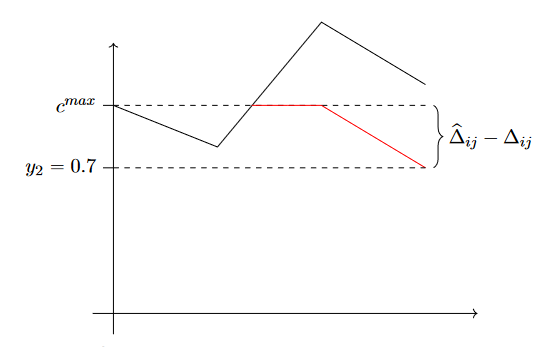
\includegraphics[width=\textwidth]{Abbildungen/Beispielgrafik.PNG}
            \source{Hier steht ggf. die Quelle}
        \end{column}
    \end{columns}
\end{frame}


\begin{frame}{Modell - so nicht!}
    \textit{Auch das Modell kann nicht ausreichend nachvollzogen werden, wenn alle Restriktionen auf einer Folie sind. Diese Folie ist daher zu voll!}
    \footnotesize
    \begin{align}
	   \min \ \sum_{i \in \mathcal{I}}\sum_{j \in \mathcal{I}} \sum_{m \in \mathcal{M}} c_{ij} \cdot X_{ijm}
    \end{align}
    u.B.d.R.
    \begin{flalign}
        \sum_{i \in \mathcal{I}} w_i \cdot Y_{im} &\le b& \forall \ m \in \mathcal{M} \\
        \sum_{j \in \mathcal{I}} X_{ijm} & = Y_{im} &  \forall \ i \in \mathcal{I}, \ m \in \mathcal{M} \\
        \sum_{i \in \mathcal{I}} X_{ijm} & = Y_{im} & \forall \ j \in \mathcal{I}, \ m \in \mathcal{M} \\
        \sum_{m \in \mathcal{M}} Y_{im} & = 1 &  \forall \ i = 2, \dots, I \\
        Z_i - Z_j + I \cdot \sum_{m \in \mathcal{M}} X_{ijm} & \le I - 1 &\forall \ i, j  = 2, \dots, I, i \neq j \\
        X_{iim} &= 0 &  \forall \ i \in \mathcal{I}, \ m \in \mathcal{M} 
    \end{flalign}
\end{frame}


\begin{frame}{Modell }
    \textit{Besser die Zielfunktion und die einzelnen Restriktionen auf mehrere Folien aufteilen. Zur  Unterstützung sollte die Notation der Zielfunktion bzw. der entsprechenden Restriktionen auf der Folie aufgenommen werden.}
    \begin{align}
	   \min \ \sum_{i \in \mathcal{I}}\sum_{j \in \mathcal{I}} \sum_{m \in \mathcal{M}} c_{ij} \cdot X_{ijm}
    \end{align}
   \vfill
    \begin{footnotesize}
        \begin{center}
            \begin{tabular}[b]{llllll}
                \toprule
                \multicolumn{4}{l|}{ \textbf{Mengen}} & \multicolumn{2}{l}{ \textbf{Parameter}}  \\
                $i, j \in \mathcal{I}$ & \multicolumn{3}{l|}{Orte mit Ort 1 als Depot}  &  $c_{ij}$ & Distanz von Ort $i$ zu Ort $j$\\
                $m \in \mathcal{M}$ & \multicolumn{3}{l|}{Touren} &    &  \\\midrule
                \multicolumn{3}{l}{ \textbf{Variablen}} & &&  \\
                \multicolumn{2}{l}{$X_{ijm} \in \{0,1\}$} & \multicolumn{4}{l}{1, wenn in Tour $m$ von Ort $i$ zu Ort $j$ gefahren wird (0 sonst)} \\
                \bottomrule
            \end{tabular}
        \end{center}
    \end{footnotesize}
\end{frame}


\begin{frame}{Modell zur Tourenplanung - Restriktionen}
    \begin{itemize}
        \item Jeder Ort (bis auf Depot) in genau einer Tour enthalten:
    \end{itemize}
    \vspace{-0.1cm}
    \begin{flalign}
        \qquad \qquad \sum_{m \in \mathcal{M}} Y_{im} & = 1 &  \forall \ i = 2, \dots, I 
    \end{flalign}
    
    \begin{itemize}
        \item Kein Ort darf sich selbst anfahren
    \end{itemize}
    \vspace{-0.1cm}
    \begin{flalign}
        \qquad \qquad X_{iim} &= 0 &  \forall \ i \in \mathcal{I}, \ m \in \mathcal{M}
    \end{flalign}    
    \vfill
    \begin{footnotesize}
        \begin{center}
            \begin{tabular}[b]{llllll}
                \toprule
                \multicolumn{4}{l}{ \textbf{Mengen}} & \multicolumn{2}{l}{ \textbf{}}  \\
                $i, j \in \mathcal{I}$ & \multicolumn{3}{l}{Orte mit Ort 1 als Depot}  &   & \\
                $m \in \mathcal{M}$ & \multicolumn{3}{l}{Touren} &    &  \\\midrule
                \multicolumn{3}{l}{ \textbf{Variablen}} & &&  \\
                \multicolumn{2}{l}{$X_{ijm} \in \{0,1\}$} & \multicolumn{4}{l}{1, wenn in Tour $m$ von Ort $i$ zu Ort $j$ gefahren wird (0 sonst)} \\
                \multicolumn{2}{l}{$Y_{im} \in \{0,1\}$} & \multicolumn{4}{l}{1, wenn Ort $i$ in Tour $m$ enthalten ist (0 sonst)} \\
                \bottomrule
            \end{tabular}
        \end{center}
    \end{footnotesize}
\end{frame}

\begin{frame}{Weitere Restriktionen}
    \textit{Wenn das Modell sehr umfangreich ist, können einige Restriktionen auch verbal erläutert werden. Ggf. können auch Gruppen von Restriktionen in einem Stichpunkt erläutert werden. Sprechen Sie die Darstellung bei Unklarheit mit Ihrer Betreuungsperson ab.}
    \begin{itemize}
        \item Beschreibung Restriktion(en) 
        \pause
        \item Beschreibung Restriktion(en)
        \pause
        \item Beschreibung Restriktion(en) 
    \end{itemize} 
\end{frame}

\begin{frame}{Tabellen}
    \textit{Bedenken Sie, dass Sie Tabellen in einer Präsentation nicht überladen. Runden Sie daher sinnvoll und stellen Sie ausgewählte Untersuchungen dar.}
    \vspace{2em}
    \begin{table}[]
        \begin{tabular}{ll|c|rrr|rrr}
        \toprule
        & & & \multicolumn{3}{c|}{\textbf{Modell 1}} & \multicolumn{3}{c}{\textbf{Modell 2}} \\
        & &\textbf{\# Instanzen} & $\boldsymbol{\overline{t}}$ & $\boldsymbol{\Tilde{t}}$ & $\overline{\text{\textbf{gap}}}$ & $\boldsymbol{\overline{t}}$ & $\boldsymbol{\Tilde{t}}$ & $\overline{\text{\textbf{gap}}}$ \\
        \hline
        \multirow{2}{*}{\textbf{klein}} & \textbf{A} & 20 & \np[s]{3.2} & \np[s]{4.2} & \np[\%]{0} & \np[s]{10.8} & \np[s]{11.9} & \np[\%]{0}\\
        & \textbf{B} & 20 & \np[s]{7.1} & \np[s]{6.9} & \np[\%]{0} & \np[s]{35.2} & \np[s]{40.5} & \np[\%]{0.6} \\
        \hline
        \multirow{2}{*}{\textbf{groß}} & \textbf{A} & 20 & \np[h]{1.2} & \np[h]{1.4} & \np[\%]{0.7} & \np[h]{2} & \np[h]{2} & \np[\%]{5.1} \\
        & \textbf{B} & 20 &  \np[h]{1.8} & \np[h]{2} & \np[\%]{7.3} & \np[h]{2} & \np[h]{2} & \np[\%]{10.8} \\
        \bottomrule
    \end{tabular}
    \end{table}
\end{frame}

\begin{frame}{Tabelle}
    \textit{In einer Tabelle können Zeilen nacheinander eingeblendet werden. Natürlich sollten Sie nicht jede Zeile einzeln einblenden. Jedoch kann es insbesondere bei größeren Untersuchungen hilfreich sein, den Fokus zunächst auf einen bestimmten Teil der Tabelle zu legen. Denken Sie daran, dass Ihre Folien immer zu Ihrer Tonspur passen müssen.}
    \vspace{1em}
    \begin{table}
        \begin{tabular}{ll|c|rrr|rrr}
        \toprule
        & & & \multicolumn{3}{c|}{\textbf{Modell 1}} & \multicolumn{3}{c}{\textbf{Modell 2}} \\
        & &\textbf{\# Instanzen} & $\boldsymbol{\overline{t}}$ & $\boldsymbol{\Tilde{t}}$ & $\overline{\text{\textbf{gap}}}$ & $\boldsymbol{\overline{t}}$ & $\boldsymbol{\Tilde{t}}$ & $\overline{\text{\textbf{gap}}}$ \\
        \hline
        \pause
        \multirow{2}{*}{\textbf{klein}} & \textbf{A} & 20 & \np[s]{3.2} & \np[s]{4.2} & \np[\%]{0} & \np[s]{10.8} & \np[s]{11.9} & \np[\%]{0}\\
        & \textbf{B} & 20 & \np[s]{7.1} & \np[s]{6.9} & \np[\%]{0} & \np[s]{35.2} & \np[s]{40.5} & \np[\%]{0.6} \\
        \hline
        \pause
        \multirow{2}{*}{\textbf{groß}} & \textbf{A} & 20 & \np[h]{1.2} & \np[h]{1.4} & \np[\%]{0.7} & \np[h]{2} & \np[h]{2} & \np[\%]{5.1} \\
        & \textbf{B} & 20 &  \np[h]{1.8} & \np[h]{2} & \np[\%]{7.3} & \np[h]{2} & \np[h]{2} & \np[\%]{10.8} \\
        \bottomrule
    \end{tabular}
    \end{table}
\end{frame}

\begin{frame}{Abbildung}
    \textit{Oft sind grafische Abbildungen einfacher zu erfassen als große Tabellen. Arbeiten Sie daher wenn möglich mit Abbildungen.}

    \begin{figure}
    \centering
    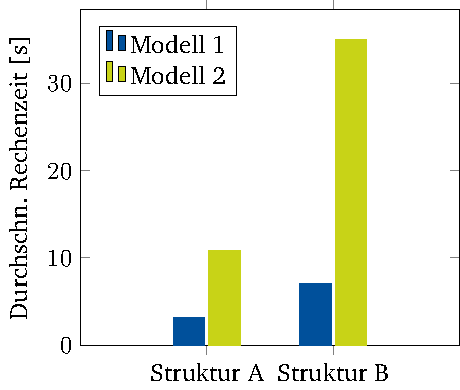
\includegraphics[width=0.45\textwidth]{Abbildungen/Bsp_Abb_Farben_1.pdf}
    \end{figure}
\end{frame}